\chapter{Структуры данных}
\section{Дерево отрезков}
Дерево отрезков (segment tree) - структура данных, позволяющая за $O(\log{n})$ времени и $O(n)$ памяти выполнять следующие операции: \newline
\begin{itemize}
\item{Подсчётфункции для отрезка $l\dots r$}
\item{Изменение одного элемента}
\item{Изменение элементов на отрезке $l\dots r$}
\end{itemize}
\subsection*{Структура дерева отрезков}
Для данного отрезка $a = [0\dots n - 1]$ начнём делить его пополам: мы получим 2 подотрезка: $a_1 = [0\cdots \frac{|a|}{2}]$ и $a_2 = [\frac{|a|}{2} + 1\cdots n - 1]$. Посчитаем сумму на них, разобьём каждый ещё на две части и проделаем всё тоже самое для полученных подотрезков. Будем делать так, пока не получим отрезки длины 1. \newline \newline
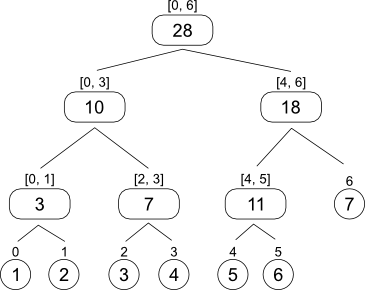
\includegraphics[height=210pt, width=400pt]{img/segment_tree} \newpage
\subsection*{Реализация дерева отрезков}
\lstinputlisting[language=C++]{src/segment_tree.cxx}
\subsection{Операции на отрезке в дереве отрезков}
/*  TODO\

  * + Надо уметь \textbf{МЕНЯТЬ} элементы\
  
  */\
  
\section{Декартово дерево}
Декартово дерево (дуча, декамида, treap, etc..) -- структура данных, в вершине которого содержится ключ $x$ и приоритет $y$ которая обладает свойством двоичного дерева поиска по ключам и свойством кучи по приоритетам. При случайных значениях приоритетов в вершинах высота дерева составит $O(\log{n})$. \newline
Рассмотрим необходимые операции:\newline

\subsection*{Объединение деревьев}
Пусть необходимо получить дерево $T$, объединив деревья $T_1$ и $T_2$. Корнем результируещего дерева станет корень одного из данных деревьев с наибольшим приоритетом. Пусть $y$ корня $T_1$ больше значения приоритета корня $T_2$. Тогда левое поддерево $T_1$ будет левым поддеревом $T$, правое дерево в таком случае будет результатом объединения правого поддерева $T_1$ с $T_2$ (т.е. описанная функция будет рекурсивной). Если на текущем шаге левое поддерево пусто, то вернем правое, аналогично и с правым. Если приоритет корня $T_2$ больше, чем у $T_1$, то делаем симметрично по аналогии. Для полученного $T$ пересчитываем нужные для запросов значения. Очевидно, глубина рекурсивных вызовов пропорцианальна высоте дерева. В декартовом дереве с большой (почти 100\%) вероятностью $h\approx\log_2{N}$, где $h$ -- высота. Тогда итоговая сложность для объединения составит $O(\log{N})$.

\subsection*{Деление деревьев по ключу}
Пусть дано дерево $T$ и ключ $x_0$. Необходимо получить такие дучи $T_l, T_r$, что в $T_l$ все ключи будут меньше $x_0$, а в $T_r$ -- больше. Пусть $k\geq x_0$, где $k$ -- ключ корня $T$, тогда левое поддерево $T_l$ совпадет с левым поддеревом $T$. Правое дерево $T_r$ будет результатом деления правого поддерева $T$ по ключу $x_0$. Также пересчитаем нужные для запросов значения для $T_r$. При $k>x_0$ действуем симметрично по аналогии. По аналогии с объединением получим сложность $O(\log{N})$.

\subsection*{Добавление узла в дучу}
Для добавления узла $x$ в дерево $T$ разделим это дерево по $x.key$ на деревья $T_l$ и $T_r$, создадим дерево $T_m$ из одного узла с ключом $x$ и случайным приоритетом $y$. Объединим деревья $T_l,T_m$, получив $T'$, исходное дерево $T$ будет результатом объединения $T'$ и $T_r$. Исходя из используемых операций сложность составит $O(\log{N})$ с большой константой.

\subsection*{Удаление  узла}
Для удаления узла с ключом $x$ из исходного дерева $T$ необходимо разделить $T$ по $x-1$, таким образом узел с ключом $x$ окажется в $T_r$ -- правом дереве после деления. Разделим $T_r$ по $x$ на $T^l_r$ и $T^r_r$. Заметим, что $T^l_r$ -- дерево, состоящие из одного узла с ключом, равным $x$. Исходное дерево без узла будет объединением $T_l$ и $T^r_r$. Сложность, аналогично с добавлением, составит $O(\log{N})$.

\section{Реализация дерамиды}
\lstinputlisting[language=C++]{src/treap.cxx}